\documentclass[11pt]{article}\usepackage[]{graphicx}\usepackage[]{color}
%% maxwidth is the original width if it is less than linewidth
%% otherwise use linewidth (to make sure the graphics do not exceed the margin)
\makeatletter
\def\maxwidth{ %
  \ifdim\Gin@nat@width>\linewidth
    \linewidth
  \else
    \Gin@nat@width
  \fi
}
\makeatother

\definecolor{fgcolor}{rgb}{0.345, 0.345, 0.345}
\newcommand{\hlnum}[1]{\textcolor[rgb]{0.686,0.059,0.569}{#1}}%
\newcommand{\hlstr}[1]{\textcolor[rgb]{0.192,0.494,0.8}{#1}}%
\newcommand{\hlcom}[1]{\textcolor[rgb]{0.678,0.584,0.686}{\textit{#1}}}%
\newcommand{\hlopt}[1]{\textcolor[rgb]{0,0,0}{#1}}%
\newcommand{\hlstd}[1]{\textcolor[rgb]{0.345,0.345,0.345}{#1}}%
\newcommand{\hlkwa}[1]{\textcolor[rgb]{0.161,0.373,0.58}{\textbf{#1}}}%
\newcommand{\hlkwb}[1]{\textcolor[rgb]{0.69,0.353,0.396}{#1}}%
\newcommand{\hlkwc}[1]{\textcolor[rgb]{0.333,0.667,0.333}{#1}}%
\newcommand{\hlkwd}[1]{\textcolor[rgb]{0.737,0.353,0.396}{\textbf{#1}}}%

\usepackage{framed}
\makeatletter
\newenvironment{kframe}{%
 \def\at@end@of@kframe{}%
 \ifinner\ifhmode%
  \def\at@end@of@kframe{\end{minipage}}%
  \begin{minipage}{\columnwidth}%
 \fi\fi%
 \def\FrameCommand##1{\hskip\@totalleftmargin \hskip-\fboxsep
 \colorbox{shadecolor}{##1}\hskip-\fboxsep
     % There is no \\@totalrightmargin, so:
     \hskip-\linewidth \hskip-\@totalleftmargin \hskip\columnwidth}%
 \MakeFramed {\advance\hsize-\width
   \@totalleftmargin\z@ \linewidth\hsize
   \@setminipage}}%
 {\par\unskip\endMakeFramed%
 \at@end@of@kframe}
\makeatother

\definecolor{shadecolor}{rgb}{.97, .97, .97}
\definecolor{messagecolor}{rgb}{0, 0, 0}
\definecolor{warningcolor}{rgb}{1, 0, 1}
\definecolor{errorcolor}{rgb}{1, 0, 0}
\newenvironment{knitrout}{}{} % an empty environment to be redefined in TeX

\usepackage{alltt}  % required first line, though can vary;
                               % this says we will use 11-point font,
                               % in the "article" format
% material beginning with the percent sign is commentary, for human
% information purposes, not processed by the LaTeX system

% these \setlength etc. lines concern page layout, amount of paragraph
% indentation etc.; beginners should ignore them (but include them)
\setlength{\oddsidemargin}{0.0in}
\setlength{\evensidemargin}{0.0in}
\setlength{\topmargin}{-0.25in}
\setlength{\headheight}{0in}
\setlength{\headsep}{0in}
\setlength{\textwidth}{6.5in}
\setlength{\textheight}{9.25in}
\setlength{\parindent}{0in}
\setlength{\parskip}{2mm}

% additional functionality can be added to LaTeX by importing packages
\usepackage{graphicx}

\title{The Binomial Distribution}
\author{Lisa Simpson}
\IfFileExists{upquote.sty}{\usepackage{upquote}}{}

\begin{document}  % required; the document starts here

\maketitle % generates a title based on the information in the preamble

The binomial distribution is a discrete probability distribution used to
model bounded counts. Specifically, a binomial random variable $x$ represents
% the $ delimiter marks the start and end of a mathematical expression
the number of successes in $n$ independent Bernoulli trials, where $p$ is
the probability of success, and $1-p$ the probability of failure.

% a blank line means a new paragraph

The probability mass function of the binomial distribution is:

\begin{equation}
	f(x | n,p) = {n \choose x} p^x (1-p)^{n-x} % note the need for braces around the n-x
\end{equation}

\noindent where $x = 0,1,2,\ldots,n$ and $p \in [0,1]$.

Applications of the binomial distribution include:

\begin{itemize} % this is an unordered list

	\item Estimation of probabilities of outcomes in any set of success or failure trials

	\item Estimation of probabilities of outcomes in games of chance

	\item Sampling of attribute

\end{itemize}

\section{Binomial sampling}

Here is a random sample from a binomial distribution with parameters $p=0.4$ and $n=20$:

\begin{knitrout}
\definecolor{shadecolor}{rgb}{0.969, 0.969, 0.969}\color{fgcolor}\begin{kframe}
\begin{alltt}
\hlstd{n} \hlkwb{<-} \hlnum{20}
\hlstd{p} \hlkwb{<-} \hlnum{0.4}
\hlcom{# Generate a random sample}
\hlstd{x} \hlkwb{<-} \hlkwd{rbinom}\hlstd{(}\hlnum{100}\hlstd{, n, p)}
\hlcom{# Generate histogram of sample}
\hlkwd{hist}\hlstd{(x,} \hlkwc{ylab} \hlstd{=} \hlstr{"Frequency"}\hlstd{,} \hlkwc{xlab} \hlstd{=} \hlstr{"X"}\hlstd{)}
\end{alltt}
\end{kframe}
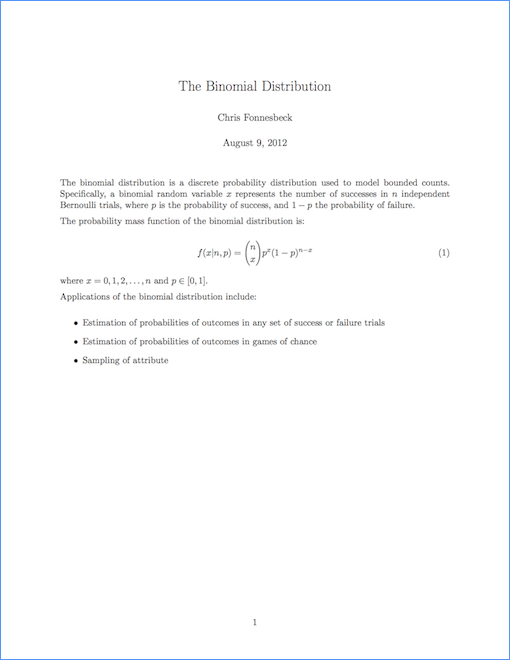
\includegraphics[width=\maxwidth]{figure/binomial} 

\end{knitrout}


\end{document}  % required; the document ends here

